\documentclass[12pt, a4paper, oneside]{article}\usepackage[]{graphicx}\usepackage[]{color}
%% maxwidth is the original width if it is less than linewidth
%% otherwise use linewidth (to make sure the graphics do not exceed the margin)
\makeatletter
\def\maxwidth{ %
  \ifdim\Gin@nat@width>\linewidth
    \linewidth
  \else
    \Gin@nat@width
  \fi
}
\makeatother

\definecolor{fgcolor}{rgb}{0.345, 0.345, 0.345}
\newcommand{\hlnum}[1]{\textcolor[rgb]{0.686,0.059,0.569}{#1}}%
\newcommand{\hlstr}[1]{\textcolor[rgb]{0.192,0.494,0.8}{#1}}%
\newcommand{\hlcom}[1]{\textcolor[rgb]{0.678,0.584,0.686}{\textit{#1}}}%
\newcommand{\hlopt}[1]{\textcolor[rgb]{0,0,0}{#1}}%
\newcommand{\hlstd}[1]{\textcolor[rgb]{0.345,0.345,0.345}{#1}}%
\newcommand{\hlkwa}[1]{\textcolor[rgb]{0.161,0.373,0.58}{\textbf{#1}}}%
\newcommand{\hlkwb}[1]{\textcolor[rgb]{0.69,0.353,0.396}{#1}}%
\newcommand{\hlkwc}[1]{\textcolor[rgb]{0.333,0.667,0.333}{#1}}%
\newcommand{\hlkwd}[1]{\textcolor[rgb]{0.737,0.353,0.396}{\textbf{#1}}}%

\usepackage{framed}
\makeatletter
\newenvironment{kframe}{%
 \def\at@end@of@kframe{}%
 \ifinner\ifhmode%
  \def\at@end@of@kframe{\end{minipage}}%
  \begin{minipage}{\columnwidth}%
 \fi\fi%
 \def\FrameCommand##1{\hskip\@totalleftmargin \hskip-\fboxsep
 \colorbox{shadecolor}{##1}\hskip-\fboxsep
     % There is no \\@totalrightmargin, so:
     \hskip-\linewidth \hskip-\@totalleftmargin \hskip\columnwidth}%
 \MakeFramed {\advance\hsize-\width
   \@totalleftmargin\z@ \linewidth\hsize
   \@setminipage}}%
 {\par\unskip\endMakeFramed%
 \at@end@of@kframe}
\makeatother

\definecolor{shadecolor}{rgb}{.97, .97, .97}
\definecolor{messagecolor}{rgb}{0, 0, 0}
\definecolor{warningcolor}{rgb}{1, 0, 1}
\definecolor{errorcolor}{rgb}{1, 0, 0}
\newenvironment{knitrout}{}{} % an empty environment to be redefined in TeX

\usepackage{alltt} % Paper size, default font size and one-sided paper
%\graphicspath{{./Figures/}} % Specifies the directory where pictures are stored
%\usepackage[dcucite]{harvard}
\usepackage{rotating}
\usepackage{amsmath}
\usepackage{setspace}
\usepackage{pdflscape}
\usepackage[flushleft]{threeparttable}
\usepackage{multirow}
\usepackage[comma, sort&compress]{natbib}% Use the natbib reference package - read up on this to edit the reference style; if you want text (e.g. Smith et al., 2012) for the in-text references (instead of numbers), remove 'numbers' 
\usepackage{graphicx}
%\bibliographystyle{plainnat}
\bibliographystyle{agsm}
\usepackage[colorlinks = true, citecolor = blue, linkcolor = blue]{hyperref}
%\hypersetup{urlcolor=blue, colorlinks=true} % Colors hyperlinks in blue - change to black if annoying
%\renewcommand[\harvardurl]{URL: \url}
 \usepackage{listings}
 \usepackage{color}
\definecolor{mygrey}{gray}{0.95}
\lstset{backgroundcolor=\color{mygrey}}
\IfFileExists{upquote.sty}{\usepackage{upquote}}{}
\begin{document}
\title{Analysis of level 4 BSc Finance and Investment results (2013-14)}
\author{Rob Hayward}
%\date{\today}
\maketitle
%\begin{abstract}
%erehrere
%\end{abstract}

The total number of students was 34.  The outcomes recorded by the summer Exam Board are in Table \ref{tabref:out}.  

% latex table generated in R 3.0.2 by xtable 1.7-1 package
% Sun Jul 20 18:47:14 2014
\begin{table}[ht]
\centering
\begin{tabular}{rr}
  \hline
 & Number of Students \\ 
  \hline
FWD &   3 \\ 
  Pass &  19 \\ 
  Refer &   6 \\ 
  Withdrawal &   6 \\ 
   \hline
\end{tabular}
\caption{Outcome of Level 4 BSc. Finance and Investsment Students} 
\label{tabref:out}
\end{table}

The figures show that 8.82 percent of the students failed and were asked to withdraw;  55.88 percent passed at the first attempt; 17.65 were referred and 17.65 withdrew before taking exams.  

There are four issues to consider in detail: the first is the proportion of students who do not complete the first year; the second is the performance of students taken onto the course through clearing; the third is the relationship between student entry grades and the level four performance; the final issue is that of the perforfmance of overseas students. 

\subsection*{Proportion of students completing level 4}

Though the University counts these fail-withdrals and withdral as the same, it is clear from an investigation of the student files that these are two distinct categories.  The second group include two students who switched to another course and it is clear that these students did not find the course to their taste 

For example, Eleanor Alabaster withdrew for``family and personal reasons'';  Erikas Gringaliunas withdrew because for financial reasons, he was an overseas student from Lithuania, had no financia support and found it too expensive in Brighton; Laura Battle withdrew because she found it impossible to keep up with the mathematical elemnts of Economics and had not settled in Brighton; Jack Bridges transfered out to Sport and Exercise Science; Craig O'Neill withdrew (Not sure look at notes); Samuel Peka transfered to Computer Science. 

I spoke to Erikas and Laura before they left.  

\subsection*{Performance of clearing students}
There were 6 students taken  onto the course through clearing. It is clear from Table \ref{tabref:out2} that these students performed relatively well.   

% latex table generated in R 3.0.2 by xtable 1.7-1 package
% Sun Jul 20 18:47:14 2014
\begin{table}[ht]
\centering
\begin{tabular}{rr}
  \hline
 & Number of Students \\ 
  \hline
FWD &   0 \\ 
  Pass &   4 \\ 
  Refer &   2 \\ 
  Withdrawal &   0 \\ 
   \hline
\end{tabular}
\caption{Outcome of Level 4 BSc. Finance and Investsment Students joined throgh clearing} 
\label{tabref:out2}
\end{table}

Using a Boxplot to compare the grade performance of all students relative to those that came through clearing (Figure \ref{fig:boxplot1}) it is evident that the weakest performance are not coming from those that were recruited through clearing.  The box plot shows the distribution of grades; the solid black line is the median grade for all students and for clearing students respectively; the box gives the interquartile range (showing the range of half the students for each group); the whiskers extent to one-and-a-half times the interquartile range; zeros are outliers that are beyond the whiskers. 

\begin{knitrout}
\definecolor{shadecolor}{rgb}{0.969, 0.969, 0.969}\color{fgcolor}\begin{figure}[]

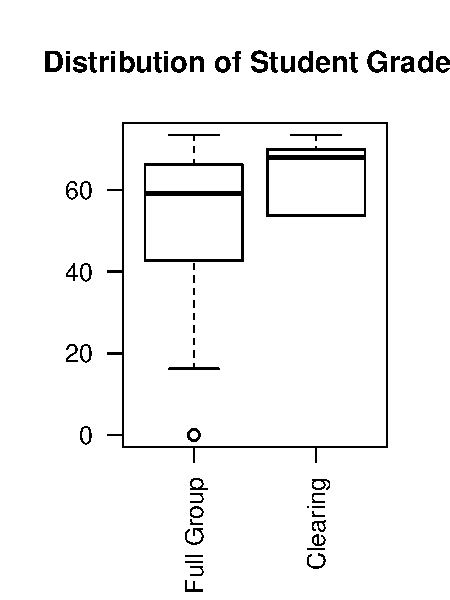
\includegraphics[width=\maxwidth]{figure/boxplot1} \caption[Comparison of total and clearing grades]{Comparison of total and clearing grades\label{fig:boxplot1}}
\end{figure}


\end{knitrout}

\subsection*{Entry grades and performance}
It is difficult to analyse the relatioknship between entry grades and student performance.  Students have been categorised into three levels of qualitifcation:  A levels that are close to the ABB course entry requirement; Other A-levels with grades below AAB; and, non-A-level, primarily BETC qualifications.  The categorisation is a little imprecise.  However, unsurprisingly, there is a strong correlation between the entry grades and the end of year result.

\begin{knitrout}
\definecolor{shadecolor}{rgb}{0.969, 0.969, 0.969}\color{fgcolor}\begin{figure}[]

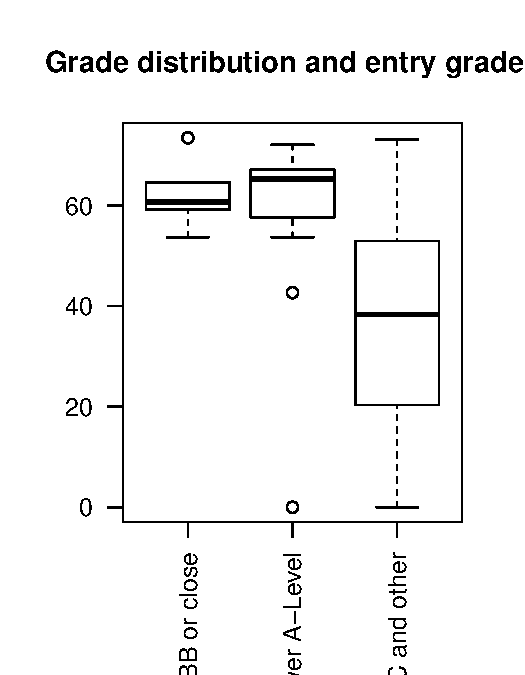
\includegraphics[width=\maxwidth]{figure/boxplot2} \caption[Entry grades and student performance]{Entry grades and student performance\label{fig:boxplot2}}
\end{figure}


\end{knitrout}


% latex table generated in R 3.0.2 by xtable 1.7-1 package
% Sun Jul 20 18:47:14 2014
\begin{table}[ht]
\centering
\begin{tabular}{rrrrr}
  \hline
 & Estimate & Std. Error & t value & Pr($>$$|$t$|$) \\ 
  \hline
da\$AlevelABB or close & 62.32 & 8.90 & 7.00 & 0.00 \\ 
  da\$AlevelLower A-Level & 58.67 & 5.14 & 11.42 & 0.00 \\ 
  da\$AlevelBTEC and other & 36.96 & 5.52 & 6.70 & 0.00 \\ 
   \hline
\end{tabular}
\caption{Level 4 grade for A-level category} 
\end{table}


\subsection*{The performance of overseas students}
These are the students with an \emph{overseas} funding category.  The boxplot, constrfcuted in the same way as outlined above, shows that the average overall level four mark for overseas students is 35.65 percent compared to 50.67 percent for the whole cohort.  

\begin{knitrout}
\definecolor{shadecolor}{rgb}{0.969, 0.969, 0.969}\color{fgcolor}
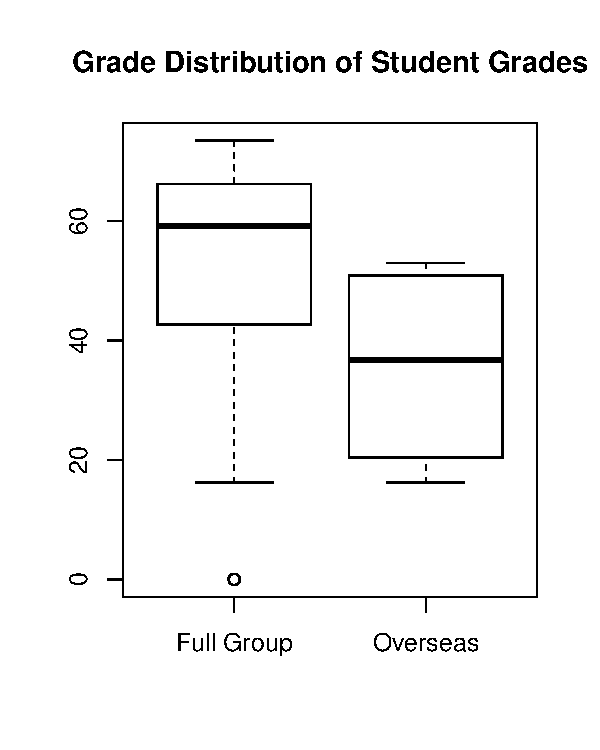
\includegraphics[width=\maxwidth]{figure/boxplot3} 

\end{knitrout}

\end{document}
